\chapter{Assignment 1: Basic Probabilities and Visualizations}

\section{Task a}

It can be said that a Binomial distribution can describe “n” number of independent Bernoulli trials, which can be also written as X ${\sim}$  B(p). We also know that the expectation of a Binomial distribution is \begin{equation}  E [X] = \sum_{k=0}^{n}kP(k)= np \label{task1_a} \end{equation} (see ~\cite{Iubh:2021}, pg. 72). \newline
Therefore, we can calculate the expectation of the Bernoulli distribution for P(vote = "for") = 0.94 where our number of trials is “n=1”. This results in the expectation of our distribution to become “p” i.e., μ = 0.94. From figure \ref{fig:task_1_a} it can be deduced that taking a single sample of voting, 94\% of the population will vote for and 6\% will vote against.

\begin{figure}[h!]
\centering
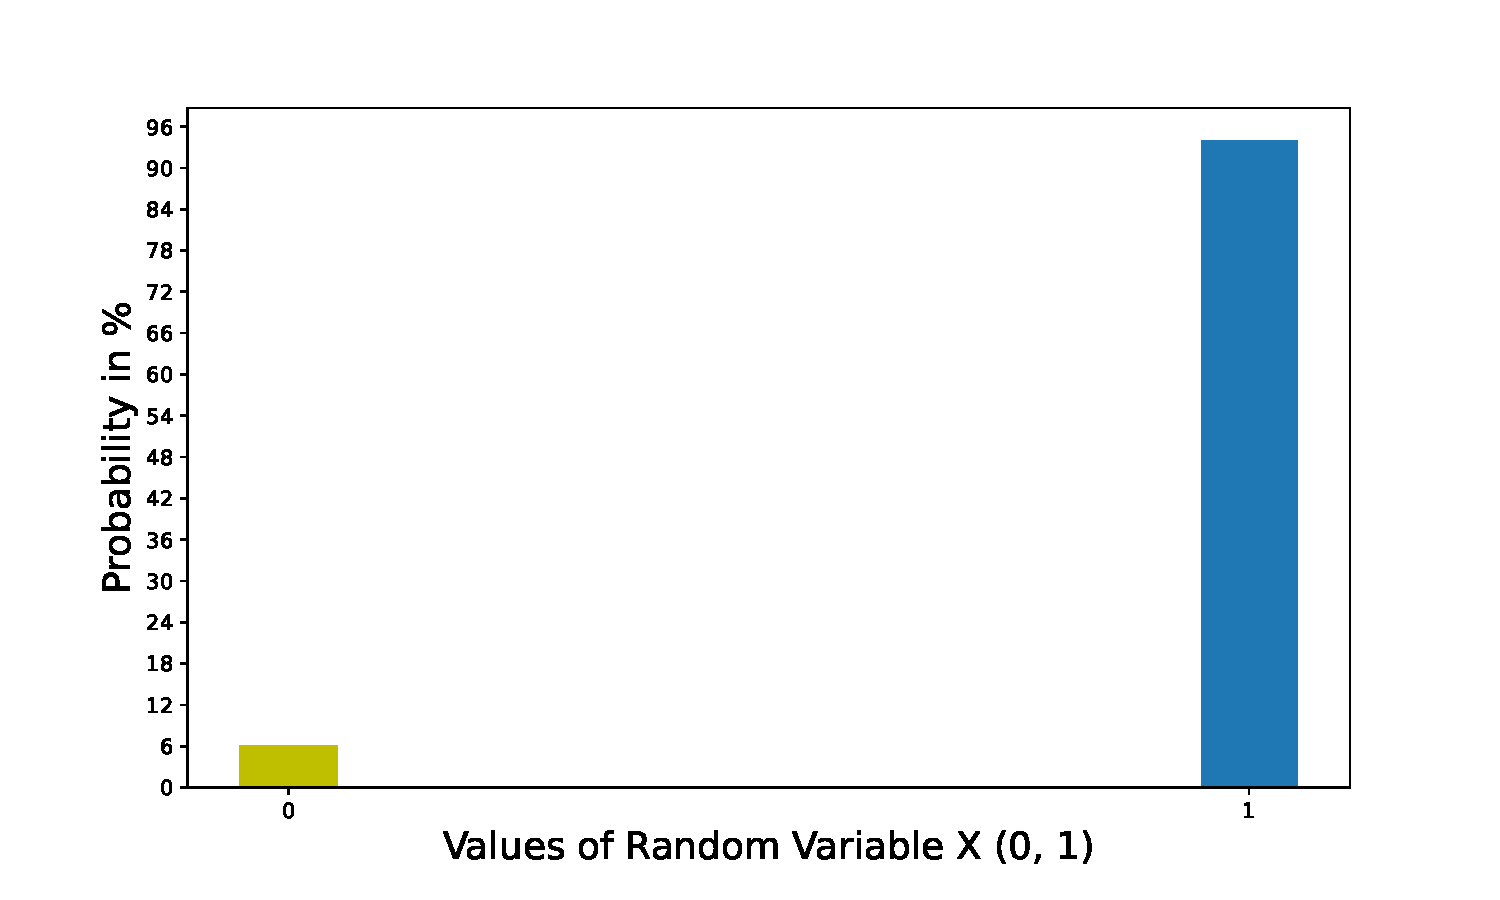
\includegraphics[width=\textwidth]{pics/task_1_a.pdf}
\caption{Bernoulli’s single trial P votes = against(6\%) \& votes=for(94\%)}\label{fig:task_1_a}
\end{figure}
\FloatBarrier 

\begin{lstlisting}[caption={: Plotting the PMF for representing Bernoulli’s single trial P (votes=for & votes = against)},label=code_task_1_a]
import matplotlib.pyplot as plt
import numpy as np

p = 0.94
# The result of the random variable is either yes or no, i.e. 0 and 1 for a Bernoulli's experiment.
X = [0, 1]

# pmf of the bernoulli single trial in %
pmf_bd_in_percent = np.array((1-p, p)) * 100

# Plot the probability distribution
fig, ax = plt.subplots(1, 1, figsize=(10, 6))

plt.xlabel("Values of Random Variable X (0, 1)", fontsize="18")
plt.ylabel("Probability in %", fontsize="18")
bar_list=plt.bar(X, pmf_bd_in_percent, width=0.1)
bar_list[0].set_color('y')
plt.xticks([0,1, 1])
plt.yticks(np.arange(0, 100, 6))

plt.savefig('images/task_1_a_matlab.pdf')
\end{lstlisting}

\section{Task b}

A Poisson distribution is mainly used to describe discrete random variable X, which gives the probability of several independent events observed over a fixed interval of time, i.e., number of people entering a supermarket in a Saturday each hour. \newline
The event of meteorites falling on the ocean each year also follows a similar pattern with the supermarket example, where the falling meteorites (discrete independent events) are observed over a year with an expectation ${\lambda}$=12. Since this random event is also observed a certain number of times in a defined time interval, we can say that Poisson is a natural candidate for such a phenomenon.\newline\newline
In Figure \ref{fig:task_1_b} we can see that the number of meteorites (k) which can fall in a year is chosen to be 22 in the distribution. Looking at the probabilities  \begin{equation} P(X=k)=\frac{\lambda^k e^{-k}}{k!}, k=0,1,2…,  \label{pmf_poission}\end{equation} when k=22 the probability of meteorites falling is less than 0.5 or 0.005. Due to this reason the k=22 is used to depict the distribution. 

\subsubsection{Median and Variance}
The variance of a Poisson distribution is given by Var[X]=$\lambda=\sigma^2$ (\cite{hogg:2005}), therefore the variance of this distribution is equal to λ parameter Var[X]=12.
Likewise, the median can be defined as the mid-point, where 50\% of the samples are either above or below this point. For this we can calculate the value of X whose cumulative sum of the probability is less than 50\%. In this case the median is also 12, which is the same as the median and variance $\lambda$. The calculation of the median or 2nd quartile is done using a for loop see (listing \ref{lst:code_task_1_b} line 21)  with the cumulative sum of the probabilities, the median is stored when a value greater than 50 is found. Instead of the value equal to 50, the value greater than is checked because it is a discrete distribution and it might not have an exact value at 50\%. Therefore, we can say that for this distribution the mean, median and variance are the same.

\begin{lstlisting}[caption={Plotting the PMF for Poisson Distribution)},label={lst:code_task_1_b}]
from scipy.stats import poisson
import numpy as np
import matplotlib.pyplot as plt

# Definitions
tick_increment = 1
lmbda = 12
n = 22
X = np.arange(0, n, 1)

mean, var, skew, kurt = poisson.stats(lmbda, moments='mvsk')

# PMF of the distribution in %
poisson_pd = poisson.pmf(X, lmbda) * 100


#Finding 2nd quartile (median) by summing the CDF and getting the value of 50%
median = 0
for i , e in enumerate(poisson_pd.cumsum()):
    if e > 50:
        median = i
        break


p_lmbda = poisson.pmf(k=var, mu=lmbda) * 100
p_median = poisson.pmf(k=median, mu=lmbda) * 100

# Plot the probability distribution
fig, ax = plt.subplots(1, 1, figsize=(20, 6))

#ax.plot(X, poisson_pd, 'bo', ms=10, label='poisson pmf')
#PMF
plt.xlabel("X - No. of Meteorites", fontsize="18")
plt.plot(X, poisson_pd, 'bo', ms=10, label='poisson pmf')
ax.vlines(X, 0, poisson_pd, colors='b', lw=5, alpha=0.5)

#Variance
plt.plot(var, p_lmbda, 'co', ms=10, label='Variance')
ax.vlines(var, 0, p_lmbda, colors='c', lw=5, alpha=0.5)

#Median
plt.plot(median, p_median, 'ro', ms=10, label='Median')
ax.vlines(median, 0, p_median, colors='r', lw=5, alpha=0.5)

plt.xticks(np.arange(0, n, tick_increment))
plt.title("Poisson Distribution - No. of Meteorites λ = 12", fontsize="18")

plt.ylabel("Probability in %", fontsize="18")
ax.grid(True)

plt.legend(loc='best', frameon=True)
plt.savefig('images/task_1_b.pdf')

\end{lstlisting}

\begin{figure}[h!]
\centering
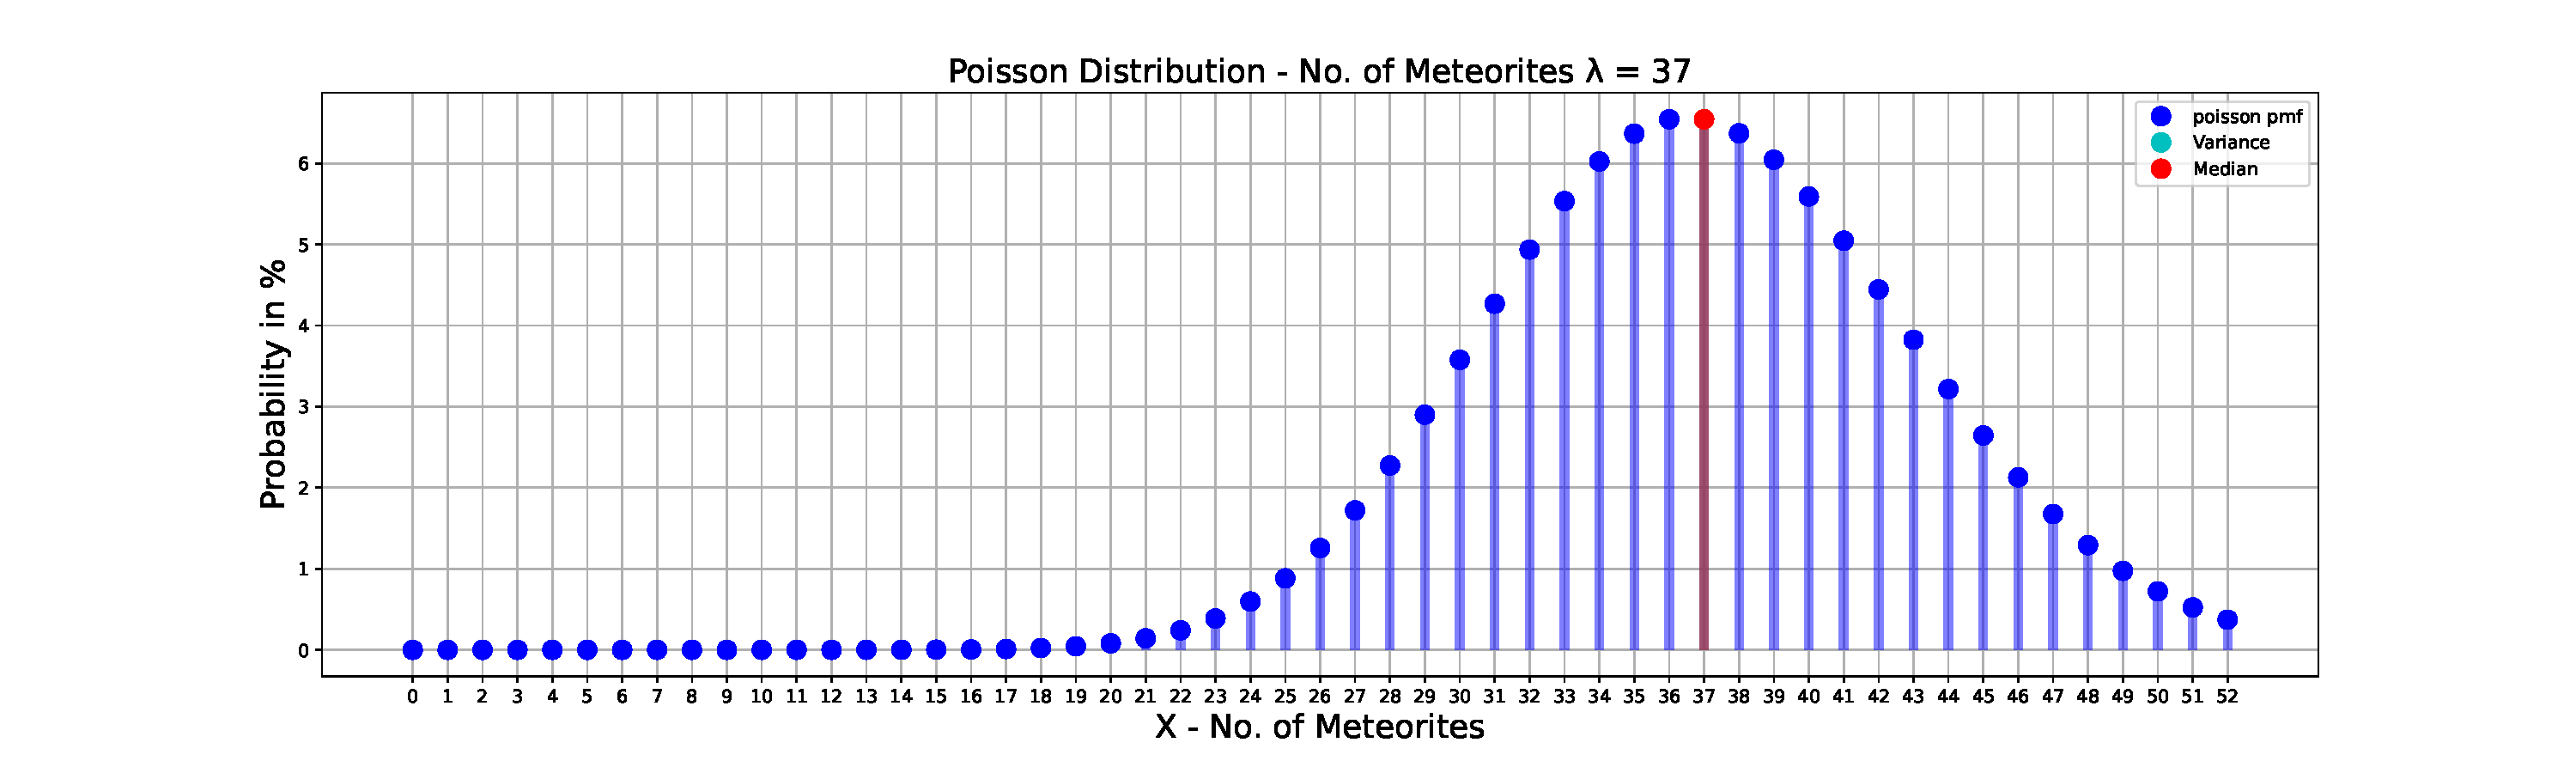
\includegraphics[width=\textwidth]{pics/task_1_b.pdf}
\caption{Poisson Distribution with k = 22 with median and variance}\label{fig:task_1_b}
\end{figure}
\FloatBarrier

\section{Task c}

Given that Y is a random variable with time to hear an owl, the probability one needs to wait to hear the owl after y hours is:
\begin{equation} \label{eqn:cdf_minus_1}
    P(Y > y) = \frac{7}{9}e^{-0.5y} + \frac{2}{9}e^{-0.25y}
\end{equation}
Since the probability given the probability of hearing the owl after y hours, this is the complementary cumulative distribution function (CCDF) P(Y $>$ y), where the CDF would be 1 minus the CCDF (see equation \ref{eqn:cdf_minus_1}). The CDF is as follows (\cite{Iubh:2021}, pg.89):
\begin{equation} \label{eqn:cdf}
    P(Y\leq y) = F(x) = 1 -(\frac{7}{9}e^{-0.5y} + \frac{2}{9}e^{-0.25y})
\end{equation}
We can obtain the probability density function by taking the first derivative of the Cumulative distribution function. The steps for the derivative are below: 
\begin{enumerate}
    \item $f(y) = \frac{\partial F}{\partial y}$
    \item $f(y)= 1- (\frac{7}{9}e^{-0.5y} + \frac{2}{9}e^{-0.25y})  \frac{\partial F}{\partial y}$
   \item $f(y)= -(\frac{7}{9}e\times -0.5e^{-0.5y} + \frac{2}{9}\times -0.25e^{-0.25y})  \frac{\partial F}{\partial y}$ 1 is removed because it is a constant
   \item $f(y)= (\frac{7}{18}e^{-0.5y} + \frac{1}{18}e^{-0.25y})$\label{eqn:pdf_exp}
\end{enumerate}
    Therefore the PDF of the function is
\begin{equation}\label{eqn:pdf_owl}
    f(y) =\begin{cases*}
    \frac{7}{18}e^{-0.5y} + \frac{1}{18}e^{-0.25y}&\text{for y$>$0}
    &\\0&\text{elsewhere}
    \end{cases*} \newline
\end{equation}
Additionally, the probability of hearing the owl lies in between the limits (2, 4] and calculated using the difference of the Probability of hearing an owl at 4 hours and 2 hours, which is as follows:

\begin{equation}
 P(2< Y \le 4) = F_{Y}(4) - F_{Y}(2)   
\end{equation}
The steps for the calculations are as follows:
\begin{enumerate}
    \item $ P(2< Y \le 4) = F_{Y}(4) - F_{Y}(2)$
    \item $ P(2< Y \le 4) = 0.813 - 0.579$ (Values for 4 and 2 are substituted in the CDF)
    \item $ P(2< Y \le 4) = 0.234$
\end{enumerate}
    
\subsubsection{Median Variance \& Quartiles}    

The mean μ can be calculated using E[Y]= $\mu$= $\int_{-\infty}^{\infty} yf(y)\,dy$. The density function f(y) used can be found in equation (\ref{eqn:pdf_owl}). Accordingly, the steps to calculate the mean are as follows: 

\begin{enumerate}
    \item E[Y] = $\int_{-\infty}^{\infty} yf(y)\,dy$
    \item E[Y] = $\int_{0}^{\infty} yf(y)\,dy$.  We can change the limits from $-\infty$ to 0 because no value exists before 0.
    \item E[Y] = $\int_{0}^{\infty} y(\frac{7}{18}e^{-0.5y} + \frac{1}{18}e^{-0.25y})\,dy$.
    \item E[Y] = $\int_{0}^{\infty} \frac{7}{18}ye^{-0.5y} + \int_{0}^{\infty} \frac{1}{18}ye^{-0.25y}\,dy$.
    \item E[Y] = $\int_{0}^{\infty} \frac{7}{18}ye^{-0.5y} + \int_{0}^{\infty} \frac{1}{18}ye^{-0.25y}\,dy$ \label{eqn:mean_line_5}
    \item E[Y] = $[\frac{7}{18}(-2ye^{-0.5y}-4e^{-0.5y})]_0^\infty + [\frac{1}{18}(-4ye^{-0.25y}-16e^{-0.25y})]_0^\infty$ Using integration by parts formula
    \item E[Y] = $[(-\frac{7}{9}ye^{-0.5y}-\frac{14}{9}e^{-0.5y})]_0^\infty + [(-\frac{2}{9}ye^{-0.25y}-\frac{8}{9}e^{-0.25y})]_0^\infty$
    \item E[Y] = $[\lim_{b\to\infty}(0)-(-\frac{7}{9}ye^{-0.5y}-\frac{14}{9}e^{-0.5y})] + [\lim_{b\to\infty}(0)-(\frac{2}{9}ye^{-0.25y}-\frac{8}{9}e^{-0.25y})]$ Applying the limits.
    \item E[Y] = $2.\overline{44}$
\end{enumerate}
Therefore the expectation of the function E[Y]=$\mu$=$2.\overline{44}$. Similarly, the variance can be calculated using the following formula Var[Y]= $\int_{-\infty}^{\infty}y^2f(y)\,dy - \mu^2$. The steps to calculate the variance are as follows: 


\begin{enumerate}
    \item E[$Y^2$] = $\int_{-\infty}^{\infty}y^2f(y)\,dy$
    \item E[$Y^2$] = $\int_{0}^{\infty} y^2f(y)\,dy$.  We can change the limits from $-\infty$ to 0 because no value exists before 0.
    \item E[$Y^2$] = $\int_{0}^{\infty} y^2(\frac{7}{18}e^{-0.5y} + \frac{1}{18}e^{-0.25y})\,dy$.
    \item E[$Y^2$] = $\int_{0}^{\infty} \frac{7}{18}y^2e^{-0.5y} + \int_{0}^{\infty} \frac{1}{18}y^2e^{-0.25y}\,dy$.
    \item E[$Y^2$] = $\int_{0}^{\infty} \frac{7}{18}y^2e^{-0.5y} + \int_{0}^{\infty} \frac{1}{18}y^2e^{-0.25y}\,dy$
    \item E[$Y^2$] = $[\frac{7}{18}(-2y^2e^{-0.5y}+4\int ye^{-0.5y})]_0^\infty + [\frac{1}{18}(-4y^2e^{-0.25y}+8\int ye^{-0.25y})]_0^\infty$ Using integration by parts formula. see above line (\ref{eqn:mean_line_5}), the integration has been already done in the step and is copied here.
    \item E[$Y^2$] = $[\frac{7}{18}(-2y^2e^{-0.5y} +4(-2ye^{-0.5y}-4e^{-0.5y})]_0^\infty + [\frac{1}{18}(-4y^2e^{-0.25y} +8(-4ye^{-0.25y}-16e^{-0.25y})]_0^\infty$
    \item E[$Y^2$] = $[\frac{7}{18}(\lim_{b\to\infty}(0)-(-2\times 0^2 \times e^{-0.5*0} +4(-2\times0e^{-0.5\times0}-4e^{-0.5\times0})] + [\frac{1}{18}(\lim_{b\to\infty}(0)-(-4\times0^2 \times e^{-0.25*0} )+8(-4\times0 \times e^{-0.25\times 0}-16e^{-0.25*0})]$
    \item E[$Y^2$] = $\frac{7}{18}\times 16 + \frac{1}{18}\times 128 = \frac{40}{3}= 13.33$
    \item Var[Y] = E[$Y^2$] - $\mu^2$ = $13.33 + 2.44^2$ = 19.28 \label{eqn:var_task_1_c}
\end{enumerate}
As calculated in line \ref{eqn:var_task_1_c} the variance is Var[Y] = 19.28. To find the quartiles one can use the CDF again, and compare it with the value of x using this the Q1(25\%) = $0.\overline{66}$ , Q1(50\%) = 1.6 and Q1(75\%) = $3.28\overline{3}$. Alternatively, one can use the inverse of the CDF $F_{Y}^{-1} (.)=x$ to also find the given quartile.

\begin{figure}[h!]
\centering
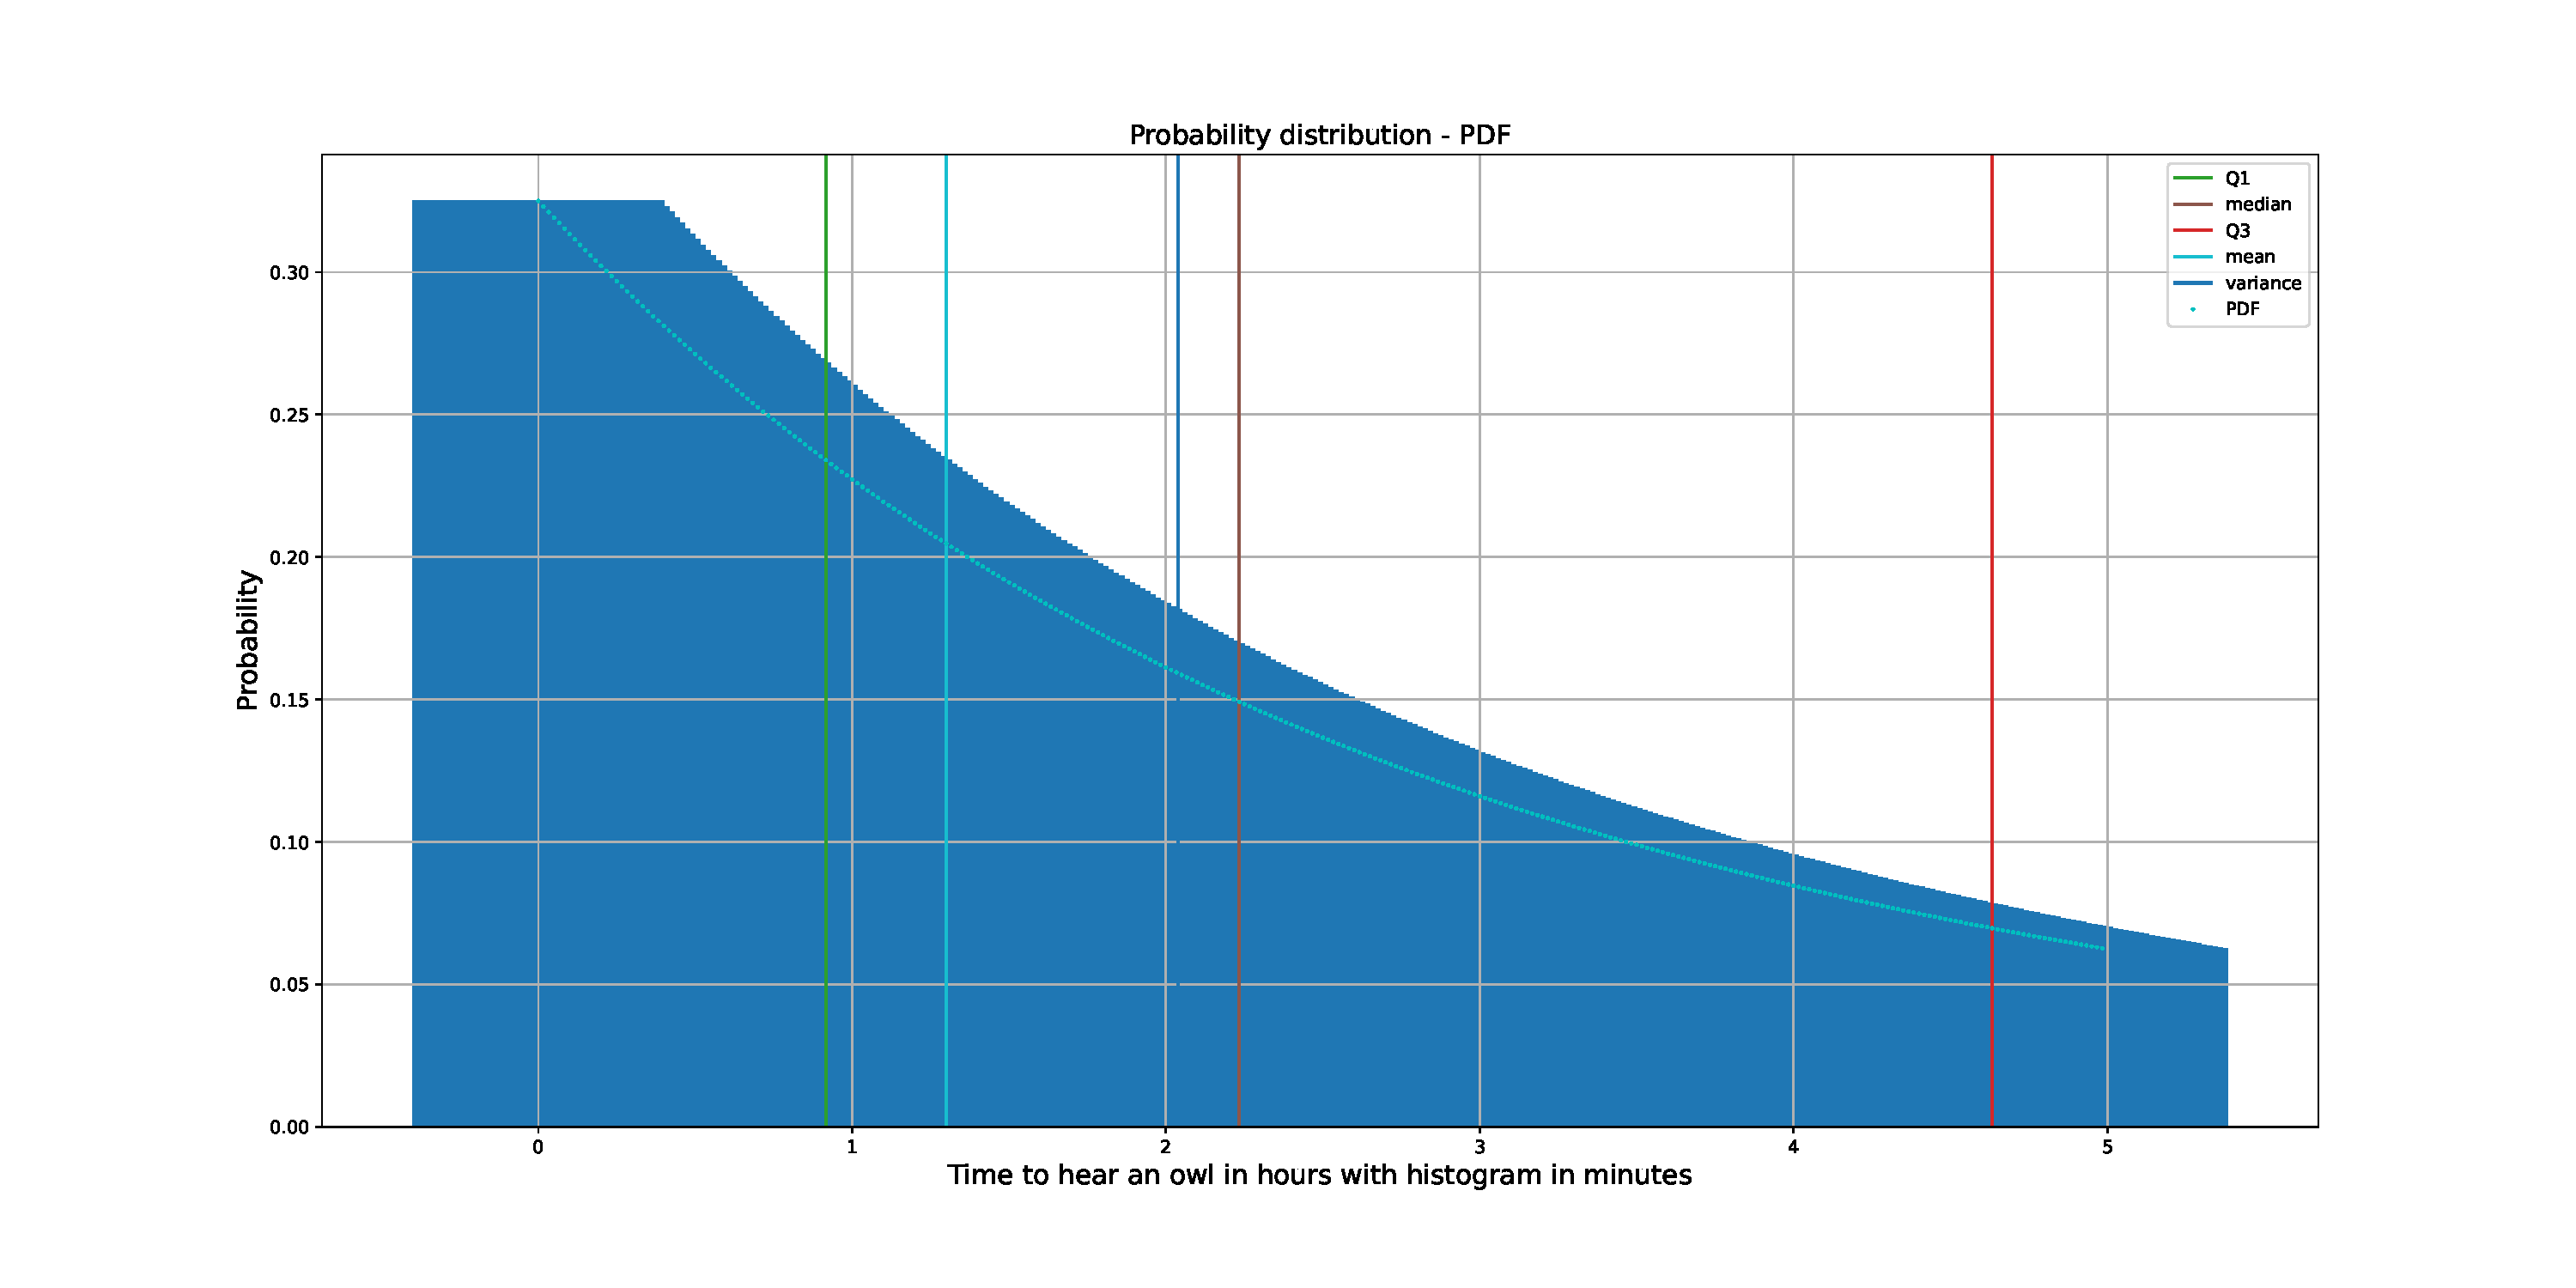
\includegraphics[width=\textwidth]{pics/task_1_c_pdf.pdf}
\caption{PDF for time to wait to hear an owl with histogram per minute (5h)}\label{fig:task_1_c}
\end{figure}
\FloatBarrier    

\begin{lstlisting}[caption={Plotting the PDF and histogram)},label={lst:code_task_1_c}]
import numpy as np
import matplotlib.pyplot as plt
from scipy.stats import rv_continuous

title_pdf = 'Probability distribution - PDF'
title_hist = r'Histogram by Minute(width = $\frac{1}{60}$  = 0.017)'
n = 5
start = 0
tick_increment = (1/60)

def my_pdf(y):
    return np.exp(y * -0.5) * (7/18) + np.exp(-0.25 * y) * (1/18)

def my_cdf(y):
    return 1 - (np.exp(y * -0.5) * (7/9) + np.exp(-0.25 * y) * (2/9))

# Function which calculates the quartiles using the points of the CDF
def calc_quartile(quartile, cdf_val, x_vals):
    #Finding quartiles by summing the CDF 50
    for index , val in enumerate(cdf_val):
        if val > quartile:
            return x_vals[index]
            break

# generate data by the minute
x = np.arange(0, n, tick_increment)
my_distribution = my_dist()
p = my_pdf(x)
cdf = my_cdf(x)

#PDF
fig, ax = plt.subplots(1, 1, figsize=(20, 10))
ax.set_title(title_pdf, fontsize=15)
ax.set_xlabel('Time to hear an owl in hours with histogram in minutes', fontsize=15)
ax.set_ylabel('Probability', fontsize=15)


# Label pdf
plt.axvline(calc_quartile(0.25, cdf, x), label='Q1', c='tab:green', linestyle='solid')
plt.axvline(calc_quartile(0.5, cdf, x), label='median', c='tab:brown', linestyle='solid')
plt.axvline(calc_quartile(0.75, cdf, x), label='Q3', c='tab:red', linestyle='solid')
plt.axvline(1.3, label='mean', c='tab:cyan', linestyle='solid')
plt.axvline(2.04, label='variance', c='tab:blue', linestyle='solid')

plt.bar(x, p)
plt.plot(x, p, 'co', ms=1, label='PDF')
ax.grid(True)
plt.legend(loc='best', frameon=True)
plt.savefig('images/task_1_c_pdf.pdf')
\end{lstlisting}


